\chapter{\ifproject%
\ifenglish Project Structure and Methodology\else โครงสร้างและขั้นตอนการทำงาน\fi
\else%
\ifenglish Project Structure\else โครงสร้างของโครงงาน\fi
\fi
}

\makeatletter

% \renewcommand\section{\@startsection {section}{1}{\z@}%
%                                    {13.5ex \@plus -1ex \@minus -.2ex}%
%                                    {2.3ex \@plus.2ex}%
%                                    {\normalfont\large\bfseries}}

\makeatother
%\vspace{2ex}
% \titleformat{\section}{\normalfont\bfseries}{\thesection}{1em}{}
% \titlespacing*{\section}{0pt}{10ex}{0pt}

\section{โครงสร้างทางสถาปัตยกรรม}

\begin{figure}[h]
\begin{center}
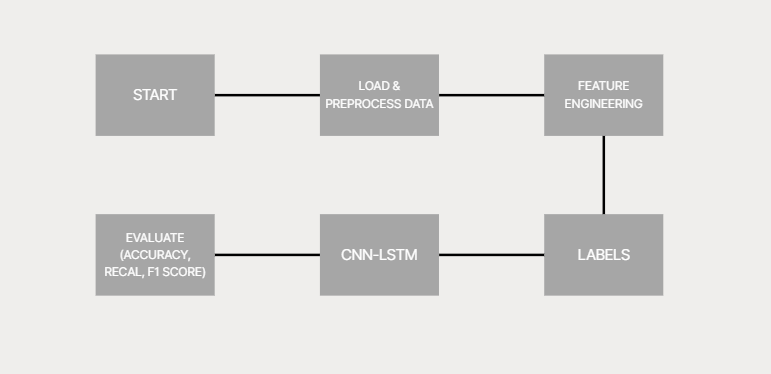
\includegraphics[width=\textwidth]{Image/System Architecture.png}
\end{center}
\caption[System Architecture]{System Architecture}
\label{fig:System Architecture}
\end{figure}

\section{การเตรียมข้อมูล (Data Preparation)}
\hspace{2em} เพื่อให้เห็นลักษณะของข้อมูลจริง ภาพนี้เป็นตัวอย่างการแสดงผลข้อมูลจาก SWaT dataset ซึ่งบันทึกค่าของเซนเซอร์และแอกชูเอเตอร์ในรูปแบบ time-series การแสดงผลในรูปแบบตารางและกราฟช่วยให้เห็นทั้งโครงสร้าง dataset และการเปลี่ยนแปลงของค่าที่เกี่ยวข้องกับเหตุการณ์ผิดปกติ (Anomaly)

\begin{figure}[h]
\begin{center}
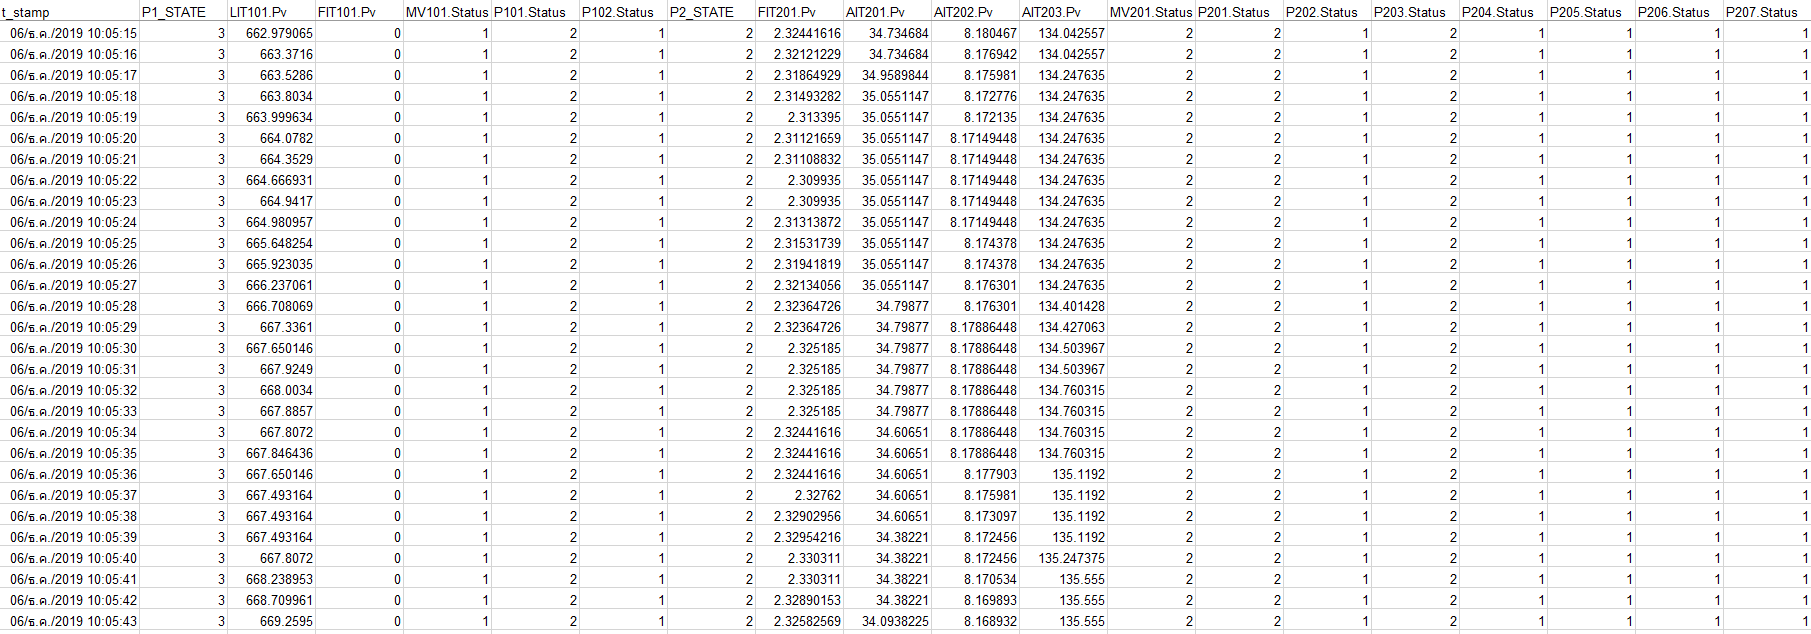
\includegraphics[width=\textwidth]{Image/dataset1.png}
\end{center}
\caption[ตัวอย่าง SWaT dataset]{ตัวอย่าง SWaT dataset จาก itrust SUTD}
\end{figure}

\begin{figure}
\begin{center}
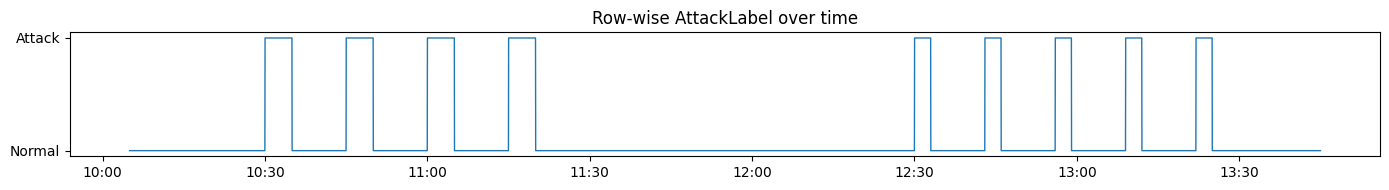
\includegraphics[width=\textwidth]{Image/dataset2.png}
\end{center}
\caption[ตัวอย่างแสดงช่วงเวลาที่โดนโจมตีภายใน dataset]{ตัวอย่างแสดงช่วงเวลาที่โดนโจมตีภายใน dataset}
\end{figure}

\subsection{การโหลดและอ่านชุดข้อมูล (Data Loading)}
\hspace{2em} ข้อมูลที่ใช้คือ SWaT Dataset ซึ่งเก็บค่าการทำงานของเซนเซอร์และแอกชูเอเตอร์ในลักษณะ time-series การโหลดข้อมูลใช้เครื่องมืออย่าง Pandas ในการอ่านไฟล์ .csv และจัดเก็บให้อยู่ในรูป DataFrame เพื่อความสะดวกต่อการวิเคราะห์และ preprocessing

\subsection{การจัดการค่าที่หายไป (Missing Value Handling)}
\hspace{2em} ข้อมูลที่ได้จากระบบ OT/ICS มักมีปัญหาค่าที่หายไป (missing values) อันเนื่องมาจากปัญหาของ sensor หรือการบันทึกข้อมูล การจัดการอาจทำได้หลายวิธี เช่น
\begin{enumerate}
  \item การลบข้อมูลแถวที่หายไป (listwise deletion)
  \item การแทนค่าด้วยสถิติ เช่น ค่าเฉลี่ย (mean) หรือค่ามัธยฐาน (median)
  \item การแทนค่าด้วยการคำนวณจากข้อมูลรอบข้าง เช่น Interpolation เหมาะกับ time-series
\end{enumerate}

\subsection{การแยกประเภทคุณลักษณะ (Continuous / Discrete Features)}
\hspace{2em} ชุดข้อมูลมักประกอบด้วยคุณลักษณะหลายประเภท เช่น
\begin{enumerate}
  \item Continuous features: ค่าจากเซนเซอร์ เช่น ความดัน อัตราการไหล ค่าการนำไฟฟ้า
  \item Discrete features: ค่าสถานะของแอกชูเอเตอร์ เช่น การเปิด/ปิดวาล์ว และการทำงานของปั๊ม
 การแยกประเภทนี้สำคัญ เนื่องจากขั้นตอน preprocessing จะแตกต่างกัน เช่น continuous ต้อง scaling แต่ discrete อาจใช้ encoding
\end{enumerate}

\subsection{การปรับสเกลข้อมูล (Scaling and Normalization)}
\hspace{2em} ค่าของเซนเซอร์บางตัวอาจอยู่ในช่วงที่ต่างกันมาก เช่น อุณหภูมิ (0–100) กับค่าแรงดัน (0–10,000) หากไม่ปรับสเกล อาจทำให้โมเดลให้ความสำคัญกับตัวแปรที่มีค่ามากเกินไป โดยใช้วิธี
\begin{center}
  Min-Max Scaling (ปรับให้อยู่ในช่วง [0,1])
\end{center}

\subsection{การแบ่งชุดข้อมูล (Training / Testing Split)}
\hspace{2em} การแบ่งชุดข้อมูลใช้หลักการ time-based split เพื่อป้องกัน data leakage โดยแบ่งเป็น
\begin{enumerate}
  \item Training set (ใช้ฝึกโมเดล)
  \item Validation set (ใช้ปรับ hyperparameter และ early stopping)
  \item Test set (ใช้ทดสอบประสิทธิภาพจริง)
\end{enumerate}
นอกจากนี้ยังใช้ Sliding Window เพื่อสร้าง sequences (window และ step) เพื่อเก็บ temporal dependency

\section{การทำ Feature Engineering}
การใช้ Sliding Window ช่วยแปลงข้อมูล time-series ให้อยู่ในรูปแบบที่โมเดลสามารถเรียนรู้ pattern ได้ โดยแต่ละ window แทนค่าลำดับข้อมูลในช่วงเวลา เช่น 180 วินาที และเลื่อนด้วย step 30 วินาที และ Correlation Heatmap เพื่อวิเคราะห์ความสัมพันธ์ระหว่าง features ซึ่งใช้เป็นแนวทางในการเลือกหรือตัดคุณลักษณะที่ซ้ำซ้อนออก

\begin{figure}[ht]
\begin{center}
      \begin{subfigure}[b]{0.9\textwidth}
            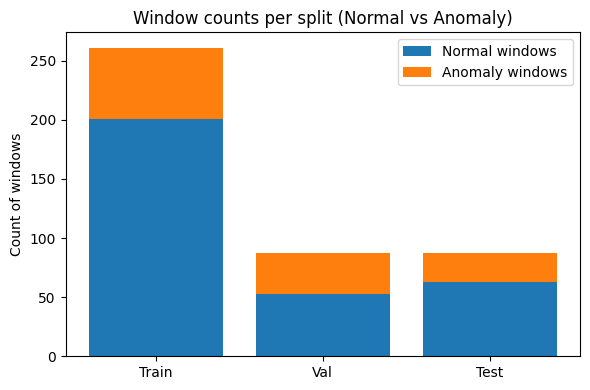
\includegraphics[width=\textwidth]{Image/window count.png}
      \end{subfigure}
          \caption[จำนวนหน้าต่างต่อช่อง (ปกติ vs ผิดปกติ)]{จำนวนหน้าต่างต่อช่อง (ปกติ vs ผิดปกติ)}
  
      \vspace{2mm}
      \begin{subfigure}[b]{\textwidth}
          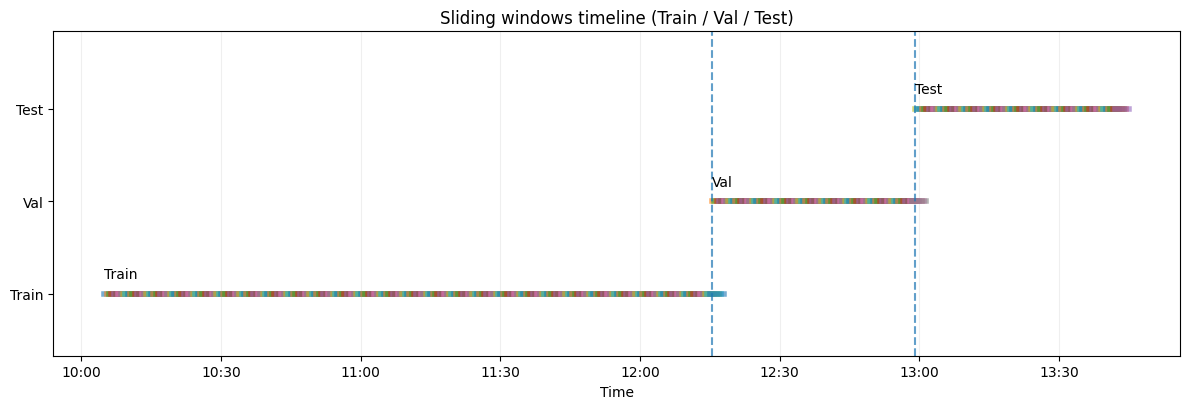
\includegraphics[width=\textwidth]{Image/slide window1.png}
      \end{subfigure}
          \caption[ไทม์ไลน์แบบหน้าต่างเลื่อน]{ไทม์ไลน์แบบหน้าต่างเลื่อน (สำหรับ Train / Val / Test)}
\end{center}
\end{figure}

\begin{figure}[ht]
\begin{center}
      \begin{subfigure}[b]{\textwidth}
          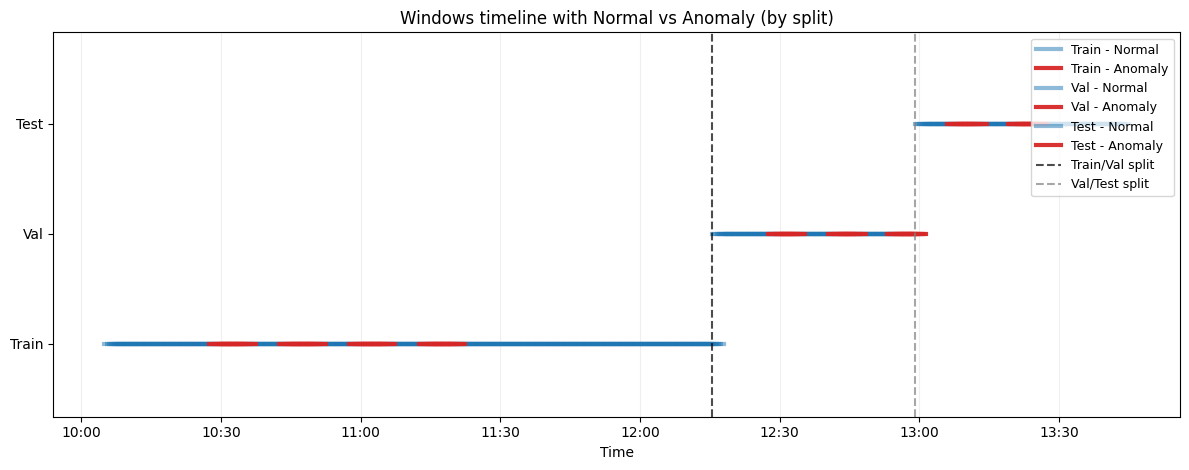
\includegraphics[width=\textwidth]{Image/slide window2.png}
    \end{subfigure}
          \caption[ไทม์ไลน์ของหน้าต่างที่แสดงข้อมูล ปกติ เทียบกับ ผิดปกติ]{ไทม์ไลน์ของหน้าต่างที่แสดงข้อมูล ปกติ เทียบกับ ผิดปกติ (แยกตามการแบ่งข้อมูล)}

    \vspace{2mm}
    \begin{subfigure}[b]{0.5\textwidth}
      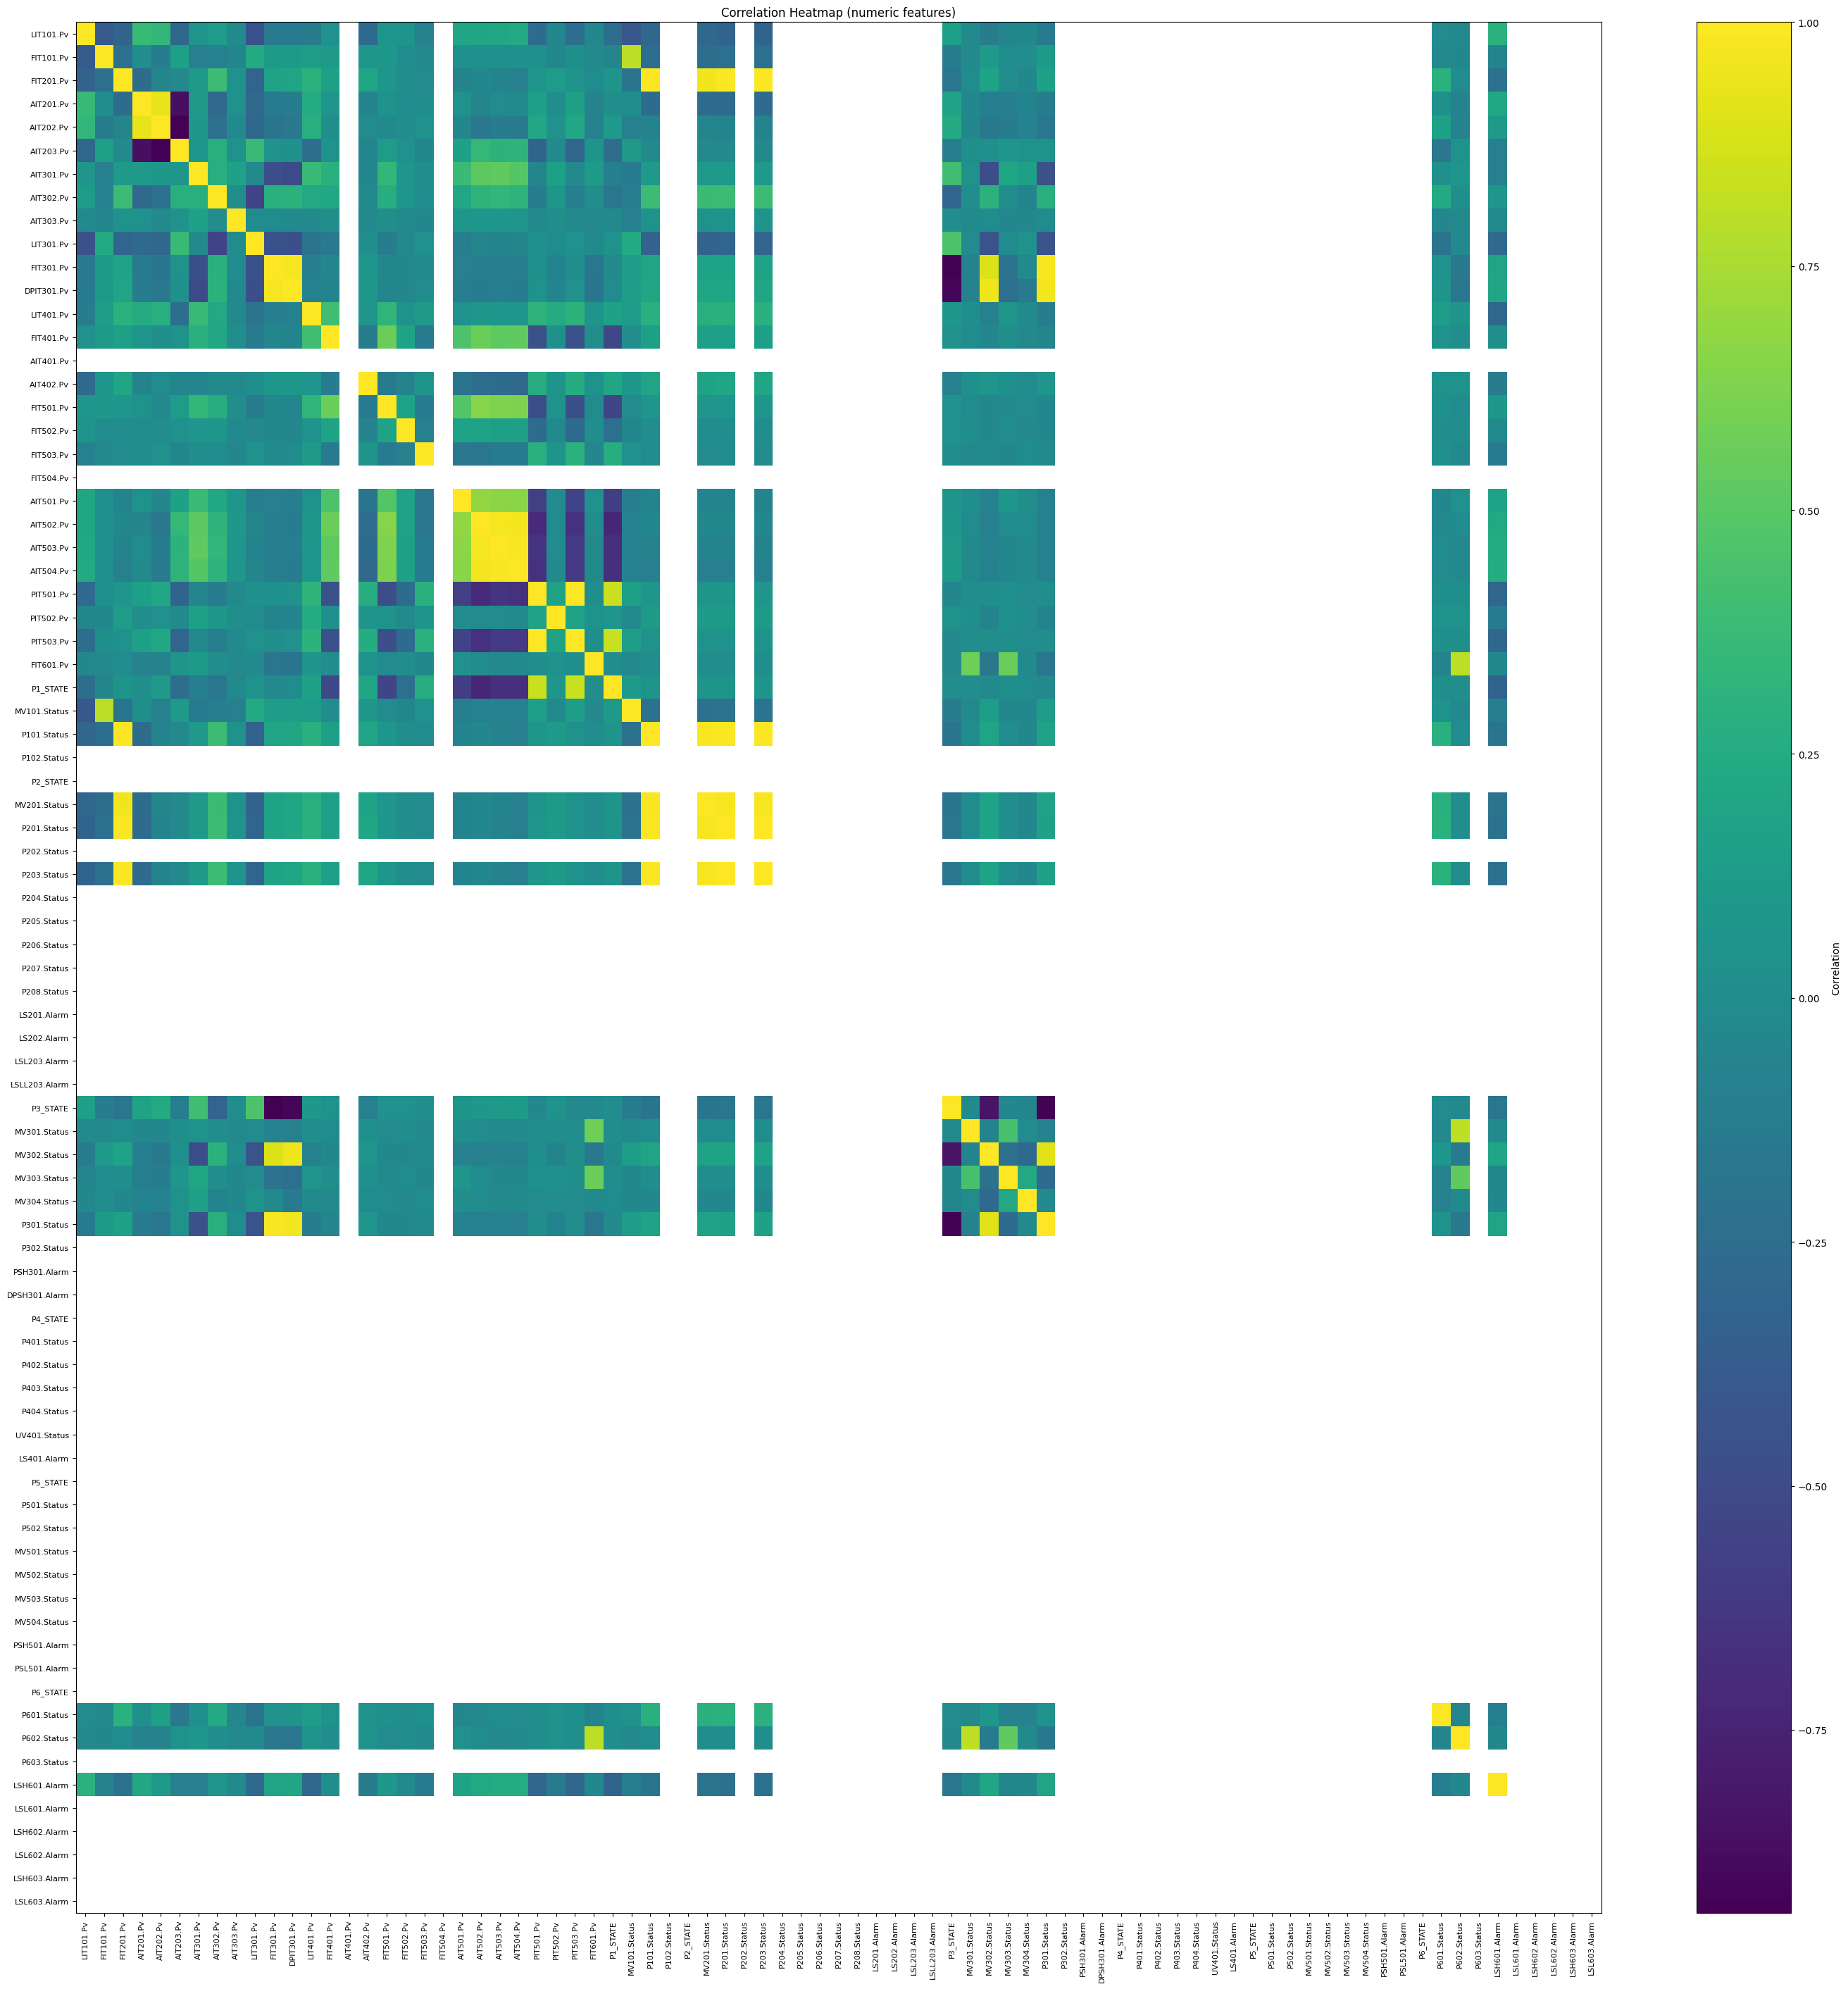
\includegraphics[width=\textwidth]{Image/heatmap.png}
    \end{subfigure}
          \caption[แผนที่ความร้อนของค่าสหสัมพันธ์]{แผนที่ความร้อนของค่าสหสัมพันธ์ (สำหรับตัวแปรเชิงตัวเลข)}
\end{center}
\end{figure}


\subsection{การเลือกคุณลักษณะที่เกี่ยวข้อง (Feature Selection)}
\hspace{2em} เพื่อให้การตรวจจับ anomaly มีประสิทธิภาพสูง ใช้วิธีเลือกคุณลักษณะ เช่น
\begin{enumerate}
  \item Correlation Matrix เพื่อตรวจหาความสัมพันธ์ระหว่าง features
  \item Mutual Information เพื่อตรวจสอบความสำคัญของแต่ละตัวแปร
\end{enumerate}

\subsection{การใช้ Sliding Window (Time-series Transformation)}
\hspace{2em} ข้อมูล time-series จาก ICS ถูกแปลงให้อยู่ในรูป Window-based Input เพื่อสร้าง sequence ที่โมเดล CNN/LSTM สามารถเรียนรู้ได้

\subsection{การสร้างคุณลักษณะใหม่ (Derived Features)}
\hspace{2em} สามารถสร้าง feature เพิ่มเติมจากข้อมูลดิบ เช่น
\begin{enumerate}
  \item ค่า moving average ของเซนเซอร์
  \item ค่าความแตกต่างระหว่างเวลา ($\Delta t$)
  \item อัตราการเปลี่ยนแปลง (derivatives)
\end{enumerate}
สิ่งเหล่านี้ช่วยให้โมเดลจับความผิดปกติได้ดีกว่าการใช้ข้อมูลดิบเพียงอย่างเดียว

\subsection{การตรวจสอบความสัมพันธ์ของคุณลักษณะ (Correlation Analysis)}
\hspace{2em} เพื่อตรวจสอบ multicollinearity หาก features มีความสัมพันธ์สูงเกินไปอาจเลือกตัดออกเพื่อลด redundancy

\section{การออกแบบและพัฒนาโมเดล (Model Design and Development)}

\subsection{การเลือกโมเดลต้นแบบ (Prototype Model)}
\hspace{2em} เลือกใช้ CNN และ LSTM เนื่องจากเหมาะกับการเรียนรู้ทั้ง local patterns (CNN) และ temporal dependency (LSTM)

\subsection{สถาปัตยกรรมของโมเดล (Model Architecture)}

\begin{figure}[h]
\begin{center}
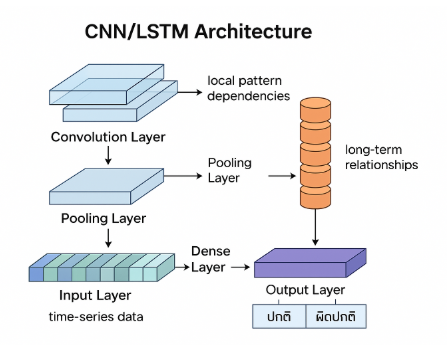
\includegraphics[width=0.5\textwidth]{Image/CNN-LSTM Arch.png}
\end{center}
\caption[CNN/LSTM Architecture]{CNN/LSTM Architecture}
\end{figure}

\begin{enumerate}
  \item Input Layer: รับข้อมูล time-series ที่ผ่าน preprocessing แล้ว
  \item Convolutional Layer: ดึง pattern ที่ซ่อนอยู่จากข้อมูล เช่น ความเปลี่ยนแปลงของ sensor
  \item Pooling Layer: ลดมิติและ noise ทำให้โมเดล generalize ได้ดีขึ้น
  \item LSTM Layer : จับความสัมพันธ์ของข้อมูลตามเวลา
  \item Fully Connected Layer: รวม feature ที่สกัดมาเพื่อใช้ในการจำแนก anomaly
  \item Output Layer: ใช้ softmax/sigmoid เพื่อตัดสินว่าเป็น “ปกติ” หรือ “ผิดปกติ”
\end{enumerate}

\subsection{การตั้งค่า Hyperparameters}
\hspace{2em} กำหนดค่าเช่น learning rate, batch size, จำนวน epoch, จำนวน filter และ kernel size ใน CNN การเลือกค่าเหล่านี้มีผลโดยตรงต่อความแม่นยำและความเร็วของการเรียนรู้

\subsection{เครื่องมือและ Framework ที่ใช้ (เช่น TensorFlow / PyTorch)}
\hspace{2em} เช่น TensorFlow, PyTorch, Scikit-learn ใช้ร่วมกับ Google Colab (GPU) เพื่อประมวลผลได้เร็วขึ้น

\section{การทดสอบและประเมินผล (Experiment and Evaluation)}

\subsection{วิธีการแบ่งชุดข้อมูลสำหรับทดสอบ (Train/Test Strategy)}
\hspace{2em} ใช้ hold-out method (train/test split) หรือ cross-validation สำหรับ time-series อาจใช้ walk-forward validation เพื่อเลียนแบบสถานการณ์จริง

\subsection{ตัวชี้วัดประสิทธิภาพ (Evaluation Metrics)}
\begin{enumerate}
  \item Accuracy: วัดความถูกต้องโดยรวม
  \item Precision, Recall, F1-score: วัดความสามารถในการตรวจจับ anomaly
  \item Detection Rate (DR), False Alarm Rate (FAR) : เน้นการวัดอัตราการตรวจจับและอัตราการแจ้งเตือนผิดพลาด
  \item Confusion Matrix, ROC-AUC, PR-AUC : วิเคราะห์เชิงลึกถึงประสิทธิภาพของโมเดล

\end{enumerate}